% Options for packages loaded elsewhere
\PassOptionsToPackage{unicode}{hyperref}
\PassOptionsToPackage{hyphens}{url}
%
\documentclass[
]{article}
\usepackage{lmodern}
\usepackage{amssymb,amsmath}
\usepackage{ifxetex,ifluatex}
\ifnum 0\ifxetex 1\fi\ifluatex 1\fi=0 % if pdftex
  \usepackage[T1]{fontenc}
  \usepackage[utf8]{inputenc}
  \usepackage{textcomp} % provide euro and other symbols
\else % if luatex or xetex
  \usepackage{unicode-math}
  \defaultfontfeatures{Scale=MatchLowercase}
  \defaultfontfeatures[\rmfamily]{Ligatures=TeX,Scale=1}
\fi
% Use upquote if available, for straight quotes in verbatim environments
\IfFileExists{upquote.sty}{\usepackage{upquote}}{}
\IfFileExists{microtype.sty}{% use microtype if available
  \usepackage[]{microtype}
  \UseMicrotypeSet[protrusion]{basicmath} % disable protrusion for tt fonts
}{}
\makeatletter
\@ifundefined{KOMAClassName}{% if non-KOMA class
  \IfFileExists{parskip.sty}{%
    \usepackage{parskip}
  }{% else
    \setlength{\parindent}{0pt}
    \setlength{\parskip}{6pt plus 2pt minus 1pt}}
}{% if KOMA class
  \KOMAoptions{parskip=half}}
\makeatother
\usepackage{xcolor}
\IfFileExists{xurl.sty}{\usepackage{xurl}}{} % add URL line breaks if available
\IfFileExists{bookmark.sty}{\usepackage{bookmark}}{\usepackage{hyperref}}
\hypersetup{
  pdftitle={DM},
  pdfauthor={Vivien \& Louis},
  hidelinks,
  pdfcreator={LaTeX via pandoc}}
\urlstyle{same} % disable monospaced font for URLs
\usepackage[margin=1in]{geometry}
\usepackage{color}
\usepackage{fancyvrb}
\newcommand{\VerbBar}{|}
\newcommand{\VERB}{\Verb[commandchars=\\\{\}]}
\DefineVerbatimEnvironment{Highlighting}{Verbatim}{commandchars=\\\{\}}
% Add ',fontsize=\small' for more characters per line
\usepackage{framed}
\definecolor{shadecolor}{RGB}{248,248,248}
\newenvironment{Shaded}{\begin{snugshade}}{\end{snugshade}}
\newcommand{\AlertTok}[1]{\textcolor[rgb]{0.94,0.16,0.16}{#1}}
\newcommand{\AnnotationTok}[1]{\textcolor[rgb]{0.56,0.35,0.01}{\textbf{\textit{#1}}}}
\newcommand{\AttributeTok}[1]{\textcolor[rgb]{0.77,0.63,0.00}{#1}}
\newcommand{\BaseNTok}[1]{\textcolor[rgb]{0.00,0.00,0.81}{#1}}
\newcommand{\BuiltInTok}[1]{#1}
\newcommand{\CharTok}[1]{\textcolor[rgb]{0.31,0.60,0.02}{#1}}
\newcommand{\CommentTok}[1]{\textcolor[rgb]{0.56,0.35,0.01}{\textit{#1}}}
\newcommand{\CommentVarTok}[1]{\textcolor[rgb]{0.56,0.35,0.01}{\textbf{\textit{#1}}}}
\newcommand{\ConstantTok}[1]{\textcolor[rgb]{0.00,0.00,0.00}{#1}}
\newcommand{\ControlFlowTok}[1]{\textcolor[rgb]{0.13,0.29,0.53}{\textbf{#1}}}
\newcommand{\DataTypeTok}[1]{\textcolor[rgb]{0.13,0.29,0.53}{#1}}
\newcommand{\DecValTok}[1]{\textcolor[rgb]{0.00,0.00,0.81}{#1}}
\newcommand{\DocumentationTok}[1]{\textcolor[rgb]{0.56,0.35,0.01}{\textbf{\textit{#1}}}}
\newcommand{\ErrorTok}[1]{\textcolor[rgb]{0.64,0.00,0.00}{\textbf{#1}}}
\newcommand{\ExtensionTok}[1]{#1}
\newcommand{\FloatTok}[1]{\textcolor[rgb]{0.00,0.00,0.81}{#1}}
\newcommand{\FunctionTok}[1]{\textcolor[rgb]{0.00,0.00,0.00}{#1}}
\newcommand{\ImportTok}[1]{#1}
\newcommand{\InformationTok}[1]{\textcolor[rgb]{0.56,0.35,0.01}{\textbf{\textit{#1}}}}
\newcommand{\KeywordTok}[1]{\textcolor[rgb]{0.13,0.29,0.53}{\textbf{#1}}}
\newcommand{\NormalTok}[1]{#1}
\newcommand{\OperatorTok}[1]{\textcolor[rgb]{0.81,0.36,0.00}{\textbf{#1}}}
\newcommand{\OtherTok}[1]{\textcolor[rgb]{0.56,0.35,0.01}{#1}}
\newcommand{\PreprocessorTok}[1]{\textcolor[rgb]{0.56,0.35,0.01}{\textit{#1}}}
\newcommand{\RegionMarkerTok}[1]{#1}
\newcommand{\SpecialCharTok}[1]{\textcolor[rgb]{0.00,0.00,0.00}{#1}}
\newcommand{\SpecialStringTok}[1]{\textcolor[rgb]{0.31,0.60,0.02}{#1}}
\newcommand{\StringTok}[1]{\textcolor[rgb]{0.31,0.60,0.02}{#1}}
\newcommand{\VariableTok}[1]{\textcolor[rgb]{0.00,0.00,0.00}{#1}}
\newcommand{\VerbatimStringTok}[1]{\textcolor[rgb]{0.31,0.60,0.02}{#1}}
\newcommand{\WarningTok}[1]{\textcolor[rgb]{0.56,0.35,0.01}{\textbf{\textit{#1}}}}
\usepackage{graphicx,grffile}
\makeatletter
\def\maxwidth{\ifdim\Gin@nat@width>\linewidth\linewidth\else\Gin@nat@width\fi}
\def\maxheight{\ifdim\Gin@nat@height>\textheight\textheight\else\Gin@nat@height\fi}
\makeatother
% Scale images if necessary, so that they will not overflow the page
% margins by default, and it is still possible to overwrite the defaults
% using explicit options in \includegraphics[width, height, ...]{}
\setkeys{Gin}{width=\maxwidth,height=\maxheight,keepaspectratio}
% Set default figure placement to htbp
\makeatletter
\def\fps@figure{htbp}
\makeatother
\setlength{\emergencystretch}{3em} % prevent overfull lines
\providecommand{\tightlist}{%
  \setlength{\itemsep}{0pt}\setlength{\parskip}{0pt}}
\setcounter{secnumdepth}{-\maxdimen} % remove section numbering

\title{DM}
\author{Vivien \& Louis}
\date{01/03/2021}

\begin{document}
\maketitle

\hypertarget{question-1}{%
\section{Question 1}\label{question-1}}

Le meilleur estimateur de \({f}(x)\) au sens de l'erreur quadratique
moyenne intégrée est l'estimateur de Parzen-Rosenblatt
\(\hat{f}(x) = \frac{1}{nh_{cv}}\sum_{j=1}^{n}K(\frac{x-X_{j}}{h_{cv}})\)
ou K est un noyau choisi et \(h_{cv}\) petit obtenue par validation
croisé \emph{leave-one-out}.

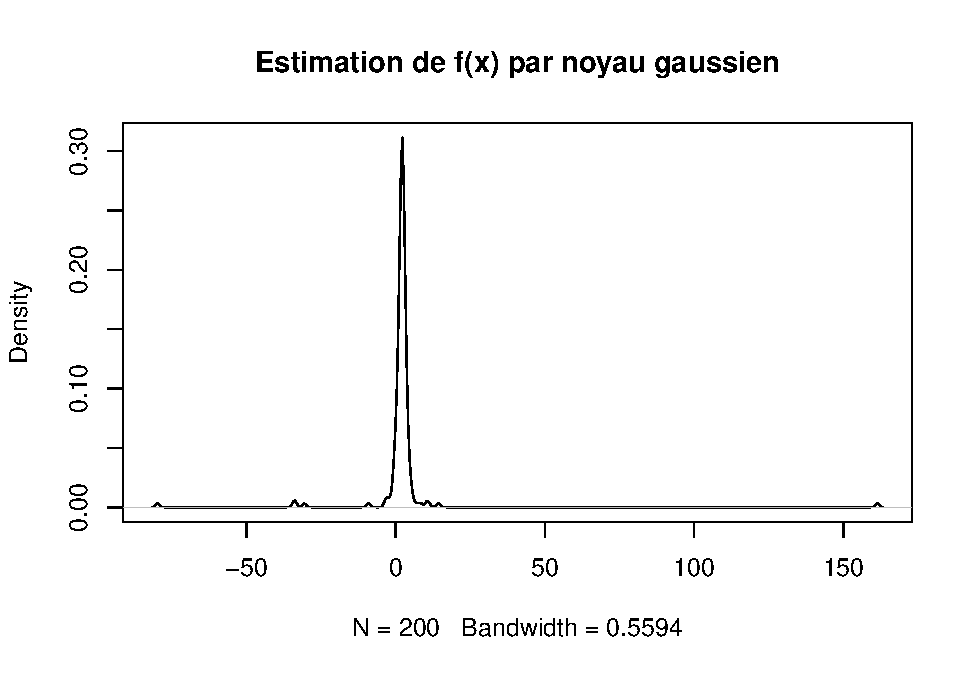
\includegraphics{DM_files/figure-latex/unnamed-chunk-2-1.pdf}
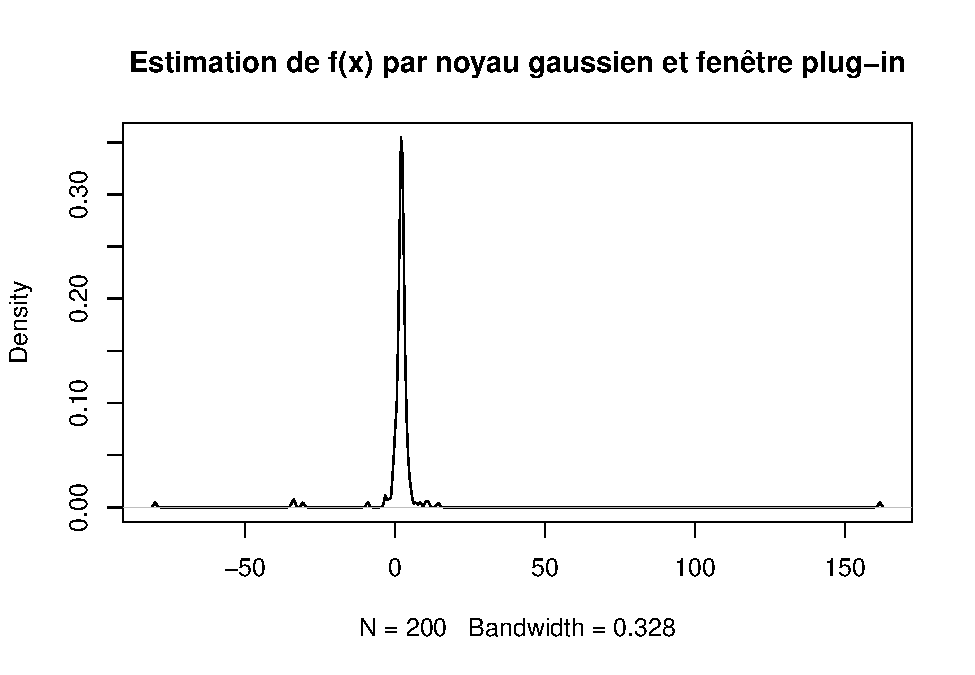
\includegraphics{DM_files/figure-latex/unnamed-chunk-2-2.pdf}
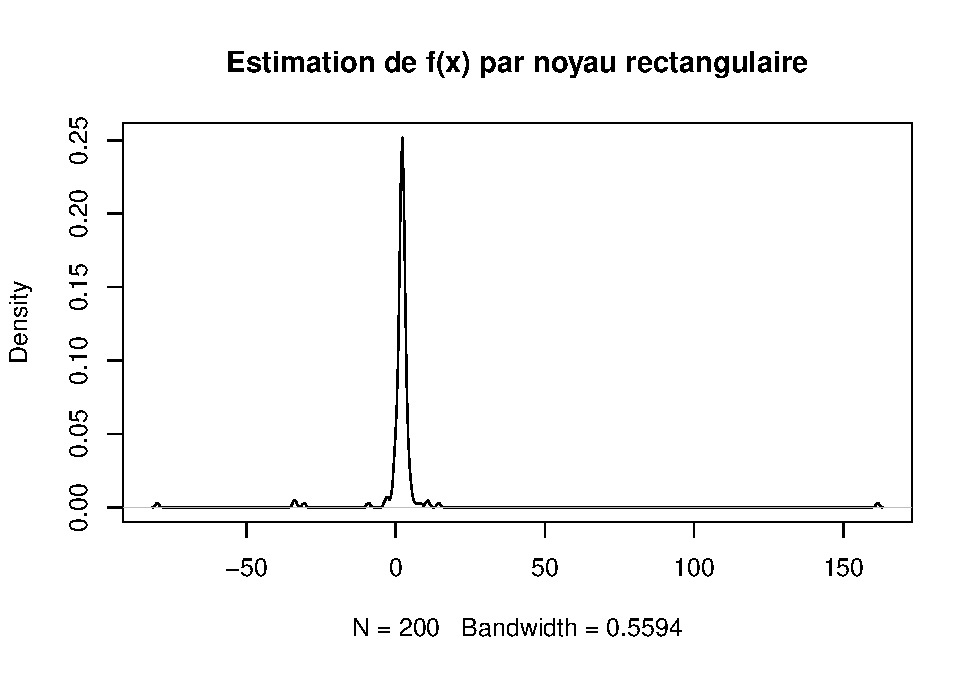
\includegraphics{DM_files/figure-latex/unnamed-chunk-2-3.pdf}
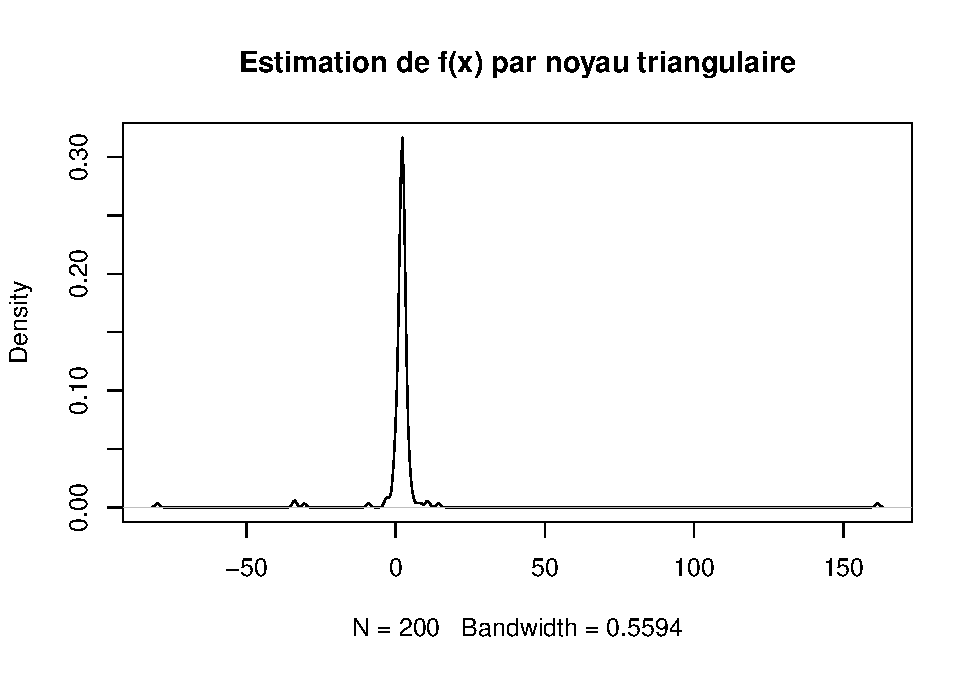
\includegraphics{DM_files/figure-latex/unnamed-chunk-2-4.pdf}
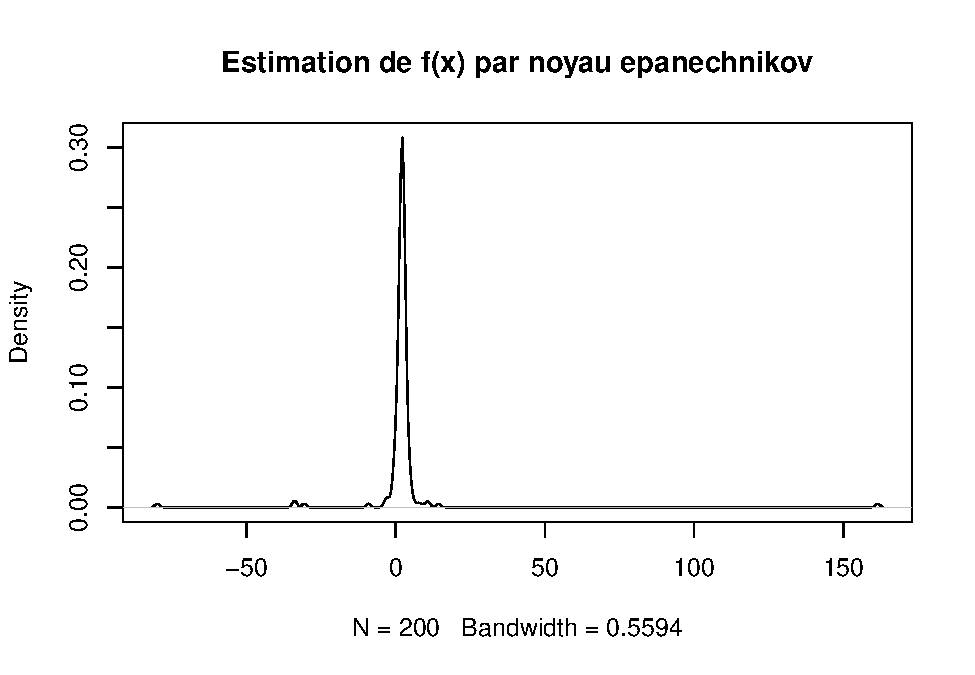
\includegraphics{DM_files/figure-latex/unnamed-chunk-2-5.pdf}
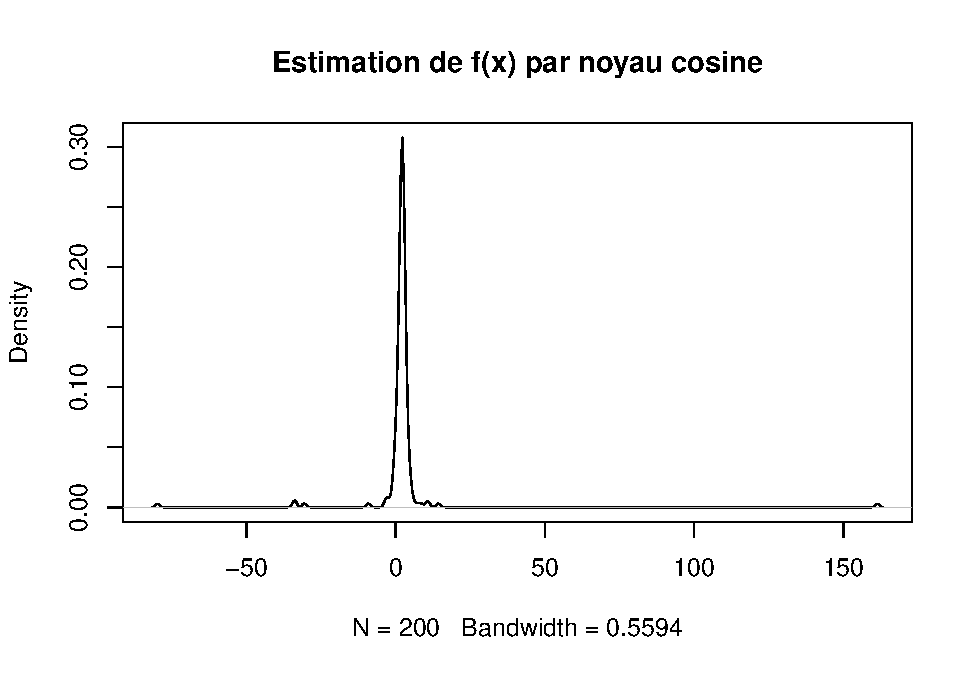
\includegraphics{DM_files/figure-latex/unnamed-chunk-2-6.pdf}
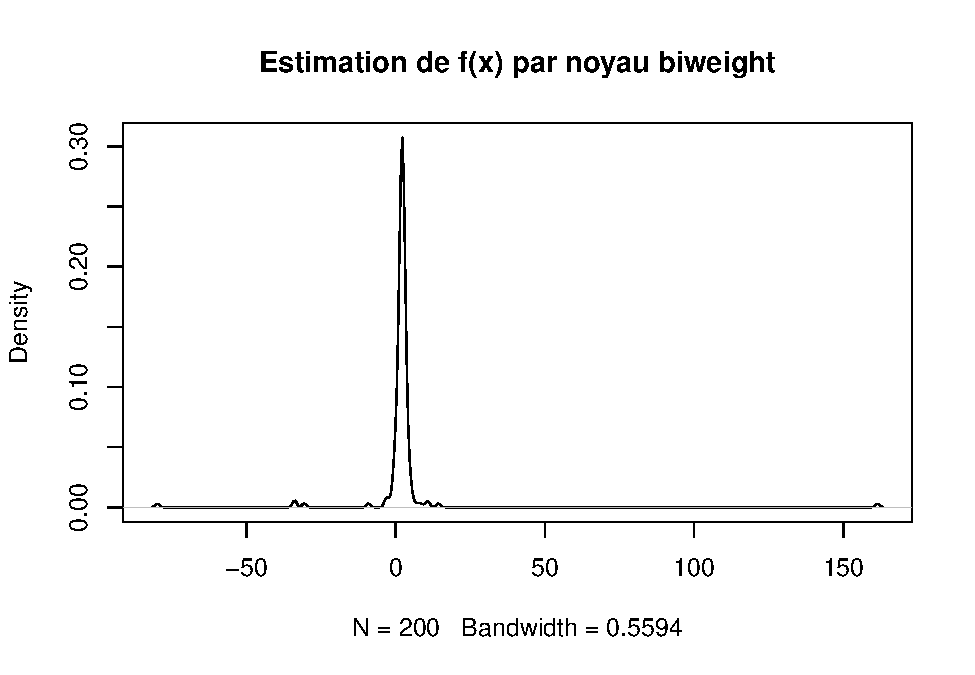
\includegraphics{DM_files/figure-latex/unnamed-chunk-2-7.pdf}

\hypertarget{question-2}{%
\section{Question 2}\label{question-2}}

\begin{itemize}
\tightlist
\item
  Puisque l'on estime une loi de densité (semblant continue de par les
  nombreux chiffres après la virgule des observations) on souhaite que
  notre estimation ait les bonnes propriétés associées aux lois de
  densité. Ainsi il vient naturellement que le noyau \(K\) doit être une
  densité de probabilité, lisse, continue et différentiable. Par défaut
  et sans information supplémentaire j'ai décidé de retenir le noyau
  gaussien. De plus, en faisant exception des valeurs extrêmes de notre
  echantillon, la partie centrale de la distribution de notre
  echantillon semble suivre une loi normale.
\end{itemize}

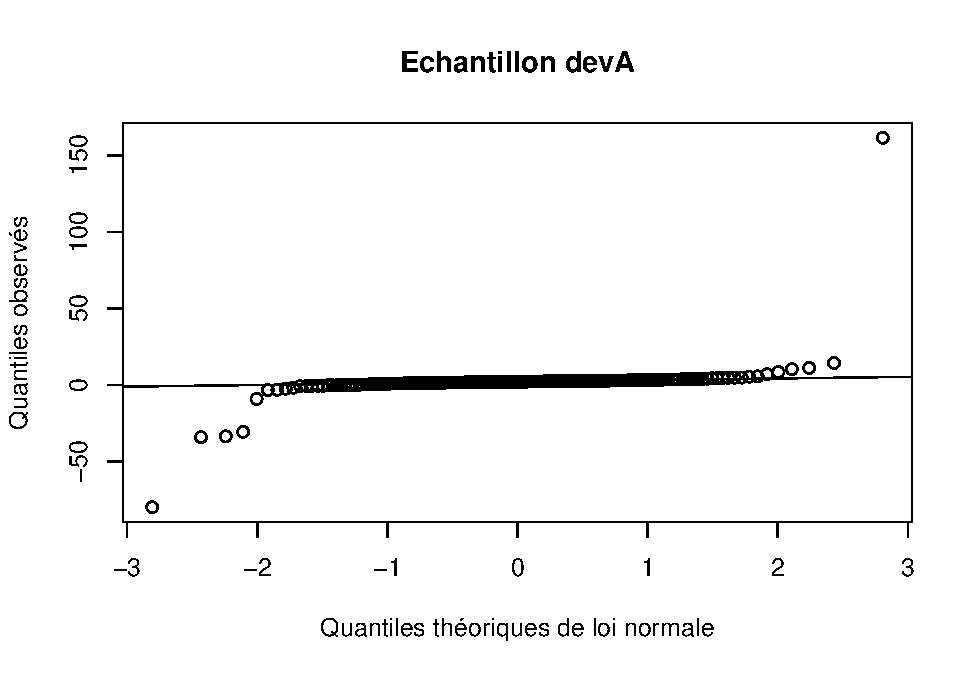
\includegraphics{DM_files/figure-latex/unnamed-chunk-3-1.pdf}

\begin{itemize}
\tightlist
\item
  Le choix de la fenêtre \(h\) est réalisé par validation croisée
  puisque
  \(h_{cv} = arg min_{h}[\int \hat{f}^2_{n}(x)dx - \frac{2}{n}\sum_{i=1}^{n}\hat{f}_{-i}(X_{i})]\).
  \(h_{}cv\) est alors égal à 0.5593725.
\end{itemize}

\hypertarget{question-3}{%
\section{Question 3}\label{question-3}}

\(f(x)\) est une loi symétrique par rapport à \(\theta_{0}\). Par
conséquent, on peut estimer graphiquement \(\theta_{0}\) par l'abscisse
du point de maximum de la courbe. \emph{i.e.}

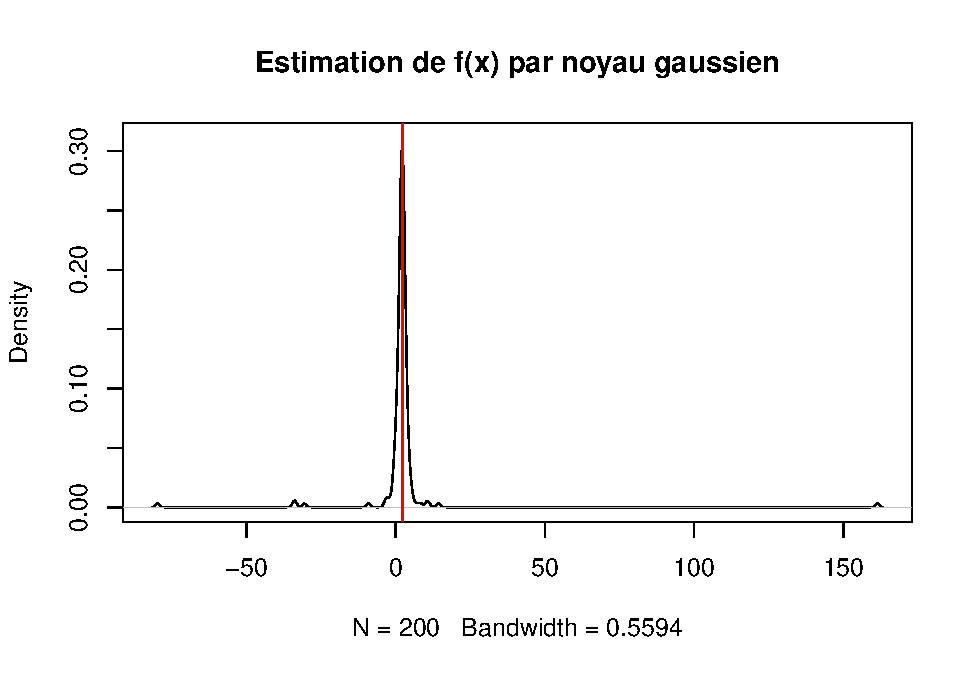
\includegraphics{DM_files/figure-latex/unnamed-chunk-4-1.pdf}
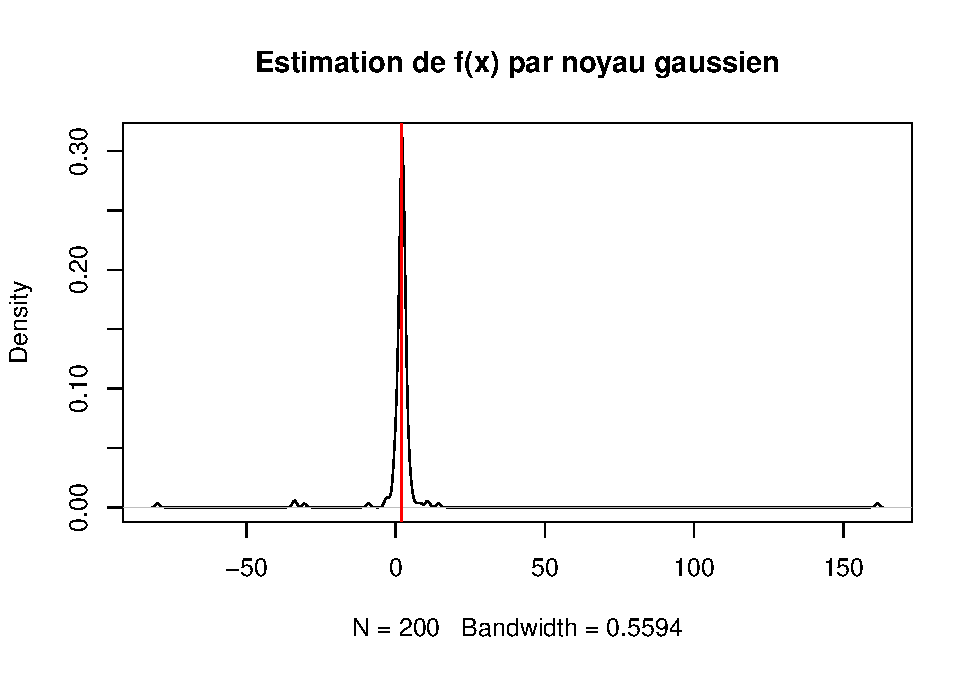
\includegraphics{DM_files/figure-latex/unnamed-chunk-4-2.pdf}

On approxime alors \(\theta_{0}\) par \(\theta_{0}^{approx} =\)
2.2656625 ou par la moyenne empirique : \(\bar{X}_{n} =\) 2.0501181
puisque que \(\theta_{0}\) est l'espérance de la loi symétrique
\(f(x)\).

\hypertarget{question-4}{%
\section{Question 4}\label{question-4}}

On peut faire mieux que ces approximations :

\#Partie B

\#Question 1

Sachant que les données observées sont issues d'une régression
linéaire,que nos valeurs manquantes sont en fait des réponses et que
l'hypothèse des observations MAR est satisfaite on a :

\(Y=m(X)+eps, E(eps|X)=0 => rho(Y,X)=Y-m(X)\) et \(Y||D,X\) si \(D=0,1\)

On souhaite estimer l'esperance de Y donc on a le systeme suivant;

\left \{

\begin{array}{rcl}
E[Y-alpha0]=0\\
D||Y,X
\end{array}
\right

=\textgreater{} \left \{

\begin{array}{rcl}
E[(D/p(X)*(Y-alpha0)]=0\\
E[(D/p(X))-1|X]=0
\end{array}
\right

\begin{Shaded}
\begin{Highlighting}[]
\KeywordTok{library}\NormalTok{(zoo)}
\end{Highlighting}
\end{Shaded}

\begin{verbatim}
## 
## Attaching package: 'zoo'
\end{verbatim}

\begin{verbatim}
## The following objects are masked from 'package:base':
## 
##     as.Date, as.Date.numeric
\end{verbatim}

\begin{Shaded}
\begin{Highlighting}[]
\NormalTok{dataB<-}\KeywordTok{read.table}\NormalTok{(}\StringTok{"C:}\CharTok{\textbackslash{}\textbackslash{}}\StringTok{Users}\CharTok{\textbackslash{}\textbackslash{}}\StringTok{admin}\CharTok{\textbackslash{}\textbackslash{}}\StringTok{Documents}\CharTok{\textbackslash{}\textbackslash{}}\StringTok{Statistique_non_parametrique}\CharTok{\textbackslash{}\textbackslash{}}\StringTok{donnees_source}\CharTok{\textbackslash{}\textbackslash{}}\StringTok{devB.txt"}\NormalTok{)}


\NormalTok{dataB}\OperatorTok{$}\NormalTok{V1<-}\KeywordTok{na.aggregate}\NormalTok{(dataB}\OperatorTok{$}\NormalTok{V1,}\DataTypeTok{fUN=}\NormalTok{median)}


\KeywordTok{plot}\NormalTok{(}\KeywordTok{ksmooth}\NormalTok{(dataB}\OperatorTok{$}\NormalTok{V2,dataB}\OperatorTok{$}\NormalTok{V1, }\DataTypeTok{kernel =} \StringTok{"normal"}\NormalTok{, }\DataTypeTok{bandwidth =}\FloatTok{0.2}\NormalTok{,}
             \DataTypeTok{range.x =} \KeywordTok{range}\NormalTok{(dataB}\OperatorTok{$}\NormalTok{V2)),}\DataTypeTok{ylim=}\KeywordTok{c}\NormalTok{(}\KeywordTok{min}\NormalTok{(dataB}\OperatorTok{$}\NormalTok{V1),}\KeywordTok{max}\NormalTok{(dataB}\OperatorTok{$}\NormalTok{V1)),}\DataTypeTok{col=}\StringTok{"red"}\NormalTok{)}
\KeywordTok{lines}\NormalTok{(}\KeywordTok{ksmooth}\NormalTok{(dataB}\OperatorTok{$}\NormalTok{V2,dataB}\OperatorTok{$}\NormalTok{V1, }\DataTypeTok{kernel =} \StringTok{"normal"}\NormalTok{, }\DataTypeTok{bandwidth =} \DecValTok{1}\NormalTok{,}
              \DataTypeTok{range.x =} \KeywordTok{range}\NormalTok{(dataB}\OperatorTok{$}\NormalTok{V2)),}\DataTypeTok{col=}\StringTok{"blue"}\NormalTok{)}
\KeywordTok{lines}\NormalTok{(}\KeywordTok{ksmooth}\NormalTok{(dataB}\OperatorTok{$}\NormalTok{V2,dataB}\OperatorTok{$}\NormalTok{V1, }\DataTypeTok{kernel =} \StringTok{"normal"}\NormalTok{, }\DataTypeTok{bandwidth =} \FloatTok{0.5}\NormalTok{,}
              \DataTypeTok{range.x =} \KeywordTok{range}\NormalTok{(dataB}\OperatorTok{$}\NormalTok{V2)),}\DataTypeTok{col=}\StringTok{"green"}\NormalTok{)}
\KeywordTok{lines}\NormalTok{(}\KeywordTok{ksmooth}\NormalTok{(dataB}\OperatorTok{$}\NormalTok{V2,dataB}\OperatorTok{$}\NormalTok{V1, }\DataTypeTok{kernel =} \StringTok{"normal"}\NormalTok{, }\DataTypeTok{bandwidth =} \DecValTok{2}\NormalTok{,}
              \DataTypeTok{range.x =} \KeywordTok{range}\NormalTok{(dataB}\OperatorTok{$}\NormalTok{V2)),}\DataTypeTok{col=}\StringTok{"skyblue"}\NormalTok{)}
\KeywordTok{lines}\NormalTok{(}\KeywordTok{ksmooth}\NormalTok{(dataB}\OperatorTok{$}\NormalTok{V2,dataB}\OperatorTok{$}\NormalTok{V1, }\DataTypeTok{kernel =} \StringTok{"normal"}\NormalTok{, }\DataTypeTok{bandwidth =} \DecValTok{5}\NormalTok{,}
              \DataTypeTok{range.x =} \KeywordTok{range}\NormalTok{(dataB}\OperatorTok{$}\NormalTok{V2)),}\DataTypeTok{col=}\StringTok{"pink"}\NormalTok{)}
\KeywordTok{abline}\NormalTok{(}\DataTypeTok{h=}\FloatTok{0.5}\NormalTok{,}\DataTypeTok{col=}\StringTok{"black"}\NormalTok{)}
\end{Highlighting}
\end{Shaded}

\includegraphics{DM_files/figure-latex/unnamed-chunk-6-1.pdf}

\end{document}
